%% ****** Start of file aiptemplate.tex ****** %
%%
%%   This file is part of the files in the distribution of AIP substyles for REVTeX4.
%%   Version 4.1 of 9 October 2009.
%%
%
% This is a template for producing documents for use with 
% the REVTEX 4.1 document class and the AIP substyles.
% 
% Copy this file to another name and then work on that file.
% That way, you always have this original template file to use.

%\documentclass[aip,graphicx]{revtex4-1}
\documentclass[aip,reprint]{revtex4-1}
\usepackage{graphicx,siunitx,pgfplots,hyperref}
\draft % marks overfull lines with a black rule on the right
\newcommand*{\pd}[3][]{%
	\frac{\partial #2}{\partial #3}
}
\newcommand*{\pdt}[2][]{%
	\frac{\partial #2}{\partial t}
}

\newcommand*{\tder}[2][]{%
	\frac{d #2}{dt}
}
\newcommand*{\ul}[2][]{%
	\underline{ #2}
}
\newcommand*{\dbul}[1]{%
	\underline{\underline{ #1}}
}
\newcommand*{\mbf}[2][]{%
	\mathbf{ #2}
}
\newcommand*{\avg}[2][]{\langle\ #2\rangle}
\newcommand*{\avgv}[2][]{\langle\mathbf{ #2}\rangle}

\newcommand*{\myvec}[1]{
	\mathbf{\underline{#1}}}
\newcommand*{\mysvec}[1]{
	\bm{\underline{#1}}}
\newcommand*{\vmom}[1]{
	n_e \langle v^{#1} \rangle}
\newcommand{\sref}[2]{Fig.\,\hyperref[#1]{\ref{#1}#2}}
%--------
\newcommand*{\vmomvec}[1]{
	n_e \langle \myvec[]{v}v^{#1} \rangle}
\newcommand{\myparallel}{{\mkern3mu\vphantom{\perp}\vrule depth 0pt\mkern2mu\vrule depth 0pt\mkern3mu}}
\newcommand{\mypara}{{
		\par\vspace{\baselineskip}}}
\def\mipath{/Users/DH814/Dropbox/IMPACT_dir/chfoil_d5/pics_modeinversion/
}
%%\newcommand{\non-localexp}{\cite{Gregori2004}\cite{Gotchev2006}\cite{Hu2008}}
\def\spvec#1{\left(\vcenter{\halign{\hfil$##$\hfil\cr \spvecA#1;;}}\right)}
\def\spvecA#1;{\if;#1;\else #1\cr \expandafter \spvecA \fi}
\DeclareSIUnit\tei{$\tau_{ei}$}
\DeclareSIUnit\vth{v_T}
\DeclareSIUnit\lmfp{$\lambda_{mfp}$}

\begin{document}

% Use the \preprint command to place your local institutional report number 
% on the title page in preprint mode.
% Multiple \preprint commands are allowed.
%\preprint{}

\title{Vlasov-Fokker-Planck simulations of pre-magnetised ablating planar targets} %Title of paper

% repeat the \author .. \affiliation  etc. as needed
% \email, \thanks, \homepage, \altaffiliation all apply to the current author.
% Explanatory text should go in the []'s, 
% actual e-mail address or url should go in the {}'s for \email and \homepage.
% Please use the appropriate macro for the type of information

% \affiliation command applies to all authors since the last \affiliation command. 
% The \affiliation command should follow the other information.

\author{D. W. Hill\email[]{dh814@ic.ac.uk}, C. P. Ridgers, R. J. Kingham, C. W. Walsh}

%\homepage[]{Your web page}
%\thanks{}
%\altaffiliation{}
\affiliation{University of York}

% Collaboration name, if desired (requires use of superscriptaddress option in \documentclass). 
% \noaffiliation is required (may also be used with the \author command).
%\collaboration{}
%\noaffiliation

\date{\today}

\begin{abstract}
	Magnetic fields, spontaneously generated around  laser heating nonuniformities have been found to invert and enhance electron pressure perturbations in the conduction zones of laser produced plasmas without applied magnetic fields \cite{Hill2018}. The application of a sufficiently strong magnetic field is predicted to damp this phenomenon, but may instead result in magneto-thermal instability. Two dimensional Vlasov-Fokker-Planck simulations of the conduction zone of laser-produced plasmas, subject to externally applied magnetic fields  of different field strengths, are performed. The effects of non-locality upon extended collisional transport terms and instability thresholds are investigated. It is found that magnetised transport terms Righi-Leduc heat flow and thermoelectric heat flow are strongly enhanced by non-locality (up to 2 fold), even at the top of the temperature gradient, due to the larger magnetisation of the mediating hot electrons (relative to their thermal counterparts). Meanwhile, the Nernst effect efficiently advects magnetic field out of the conduction zone before instability (which requires Hall parameters, $\chi >0.1$) can take hold. 
% insert abstract here
\end{abstract}
% Conventionally flux suppression occurs a
% 


\pacs{}% insert suggested PACS numbers in braces on next line

\maketitle %\maketitle must follow title, authors, abstract and \pacs

% Body of paper goes here. Use proper sectioning commands. 
% References should be done using the \cite, \ref, and \label commands
\section{Introduction}
%\label{}
The application of an external magnetic field to an  inertial-confinement-fusion (ICF) target presents a promising method of improving the neutron yield \cite{Chang2011}. 
Improvements in fusion performance are attributed to the embedded magnetic flux inhibiting heat losses. In order to attain this compressed, hot spot state, the fuel capsule must first undergo the process of laser ablation. In the ablation phase, the outer surface of the fuel capsule is ionised and heated by the laser drive, forming a rapidly expanding coronal plasma. The rapid thermal expansion causes a reactionary force, manifesting as a hydrodynamic (ablation) pressure which compresses the fuel capsule. To maintain the ablation pressure, energy must be efficiently conducted from the hot, low density plasma at the critical surface, where the energy is absorbed, to the ablation surface, the point of peak pressure at the cold, solid density target surface. The presence of an external magnetic field may both inhibit thermal conduction in this region, perpendicular to the field direction, \cite{Braginskii1965}, and seed field-generating thermal \cite{Fruchtman1992} and magneto-thermal \cite{Bissell2010a} instabilities around inhomogeneities in the laser-energy deposition.

It has long been known that the conditions within this conduction zone, the region between the critical and ablation surfaces, are far from local thermodynamic equilibrium (LTE) \cite{Bell1981}.  The collisional mean-free-paths of the heat carrying electrons are on the order of the temperature scale length, $L_T= T_{e,0}/\partial_x T_{e,0}$. The electron thermal transport is non-local; the thermal conduction cannot be described by a Fick-type law, dependent only on the local temperature gradient, $\nabla T_e$, and the Braginskii thermal conductivity, $\kappa$ \cite{Braginskii1965}: $\mathbf{q} = -\kappa \nabla T_e$. Magnetic fields strongly effect non-locality and vice versa \cite{Brantov2003,Ridgers2008,Hill2018} and their interplay in magnetised ICF implosions is poorly understood \cite{Davies2015}.

Previously it was shown that magnetic fields spontaneously generated around nonuniformities in the laser absorption could result in an inversion and enhancement of pressure perturbations  within the conduction zone \cite{Hill2018}. The phenomenon was due to the sideways deflection of the heat flow in the conduction zone by the magnetic field, the Righi-Leduc effect. For sufficiently strong Hall parameters ($\chi \gtrsim 0.1$), the direction of Righi-Leduc heat flow reverses along magnetisation gradients. It is predicted that under such conditions phase inversion should be suppressed. These conditions, however, may instead result in instability \cite{Fruchtman1992,Bissell2010a}. Nevertheless, the true conduction zone dynamics remain unclear, as assumptions included in instability growth rate calculations are not valid in the steep gradients of the conduction zone.


In this paper we present 2D Vlasov-Fokker-Planck simulations of a planar, ablating CH foil, subject to an externally applied, out-of-plane magnetic field.  Three applied magnetic field strengths are used, $\SI{0}{T}$, $\SI{50}{T}$ and $\SI{400}{T}$. The laser heating profile is modulated with a transverse sinusoidal perturbation which takes the form $I(x) = I_0(x)(1 + \alpha e^{i(2\pi y/\lambda_p})$ and the perturbation wavelength is $\lambda_p = \SI{5}{\micro\meter}$. Modulations between 1\% - 100\% ($\alpha = 0.01-1$) are examined. The phenomenology between the two limits are similar, thus in general only the 1\% case will be discussed here.  In Sections \ref{sec:1D} the effects of non-locality on the transport are examined in one-dimension. In Section \ref{sec:2D} the effects of applied magnetic field upon the perturbation evolution is investigated. Finally, the effects of non-locality on transverse heat-flow is examined in Section \ref{sec:non-locality-2D}.

\section{Theoretical Background}

% Theoretical background

The dynamics of electrons in a semi-collisional plasma is well described by the Vlasov-Fokker-Planck equation,
\begin{eqnarray}
&\left[\frac{\partial}{\partial t}+ \mathbf{v}\cdot \frac{\partial}{\partial \mathbf{r}} + \frac{e}{m_e}\left( \mathbf{E} +  \mathbf{v} \times  \mathbf{B} \right ) \cdot  \frac{\partial}{\partial \mathbf{v}} \right] f( \mathbf{v},\mathbf{r},t) =
\nonumber\\ 
-  &\frac{\partial}{\partial \mathbf{v}} \cdot \left\{ f( \mathbf{v},\mathbf{r},t) \langle \Delta \mathbf{v} \rangle \right\} + \frac{1}{2} \frac{\partial}{\partial \mathbf{v}} \frac{\partial}{\partial \mathbf{v}}:  \left\{ f( \mathbf{v},\mathbf{r},t) \langle \Delta \mathbf{v} \Delta \mathbf{v}\rangle \right\}, \label{eq:VFP}
\end{eqnarray}
where $\mathbf{E}$ and $\mathbf{B}$ represent the macroscopic electric and magnetic fields. In order to make  this equation more tractable it is standard to expand the electron distribution function, $f( \mathbf{v},\mathbf{r},t)$, in Cartesian tensors \cite{Shkarovsky1966}, $f(\mathbf{v},\mathbf{r},t) = f_0(v,\mathbf{r},t) + \myvec{f}_1(v,\mathbf{r},t) \cdot \hat{\mathbf{v}} + \dots$ (where $\hat{\mathbf{v}}$ is the velocity unit vector). Higher order terms in this expansion represent increasing degrees of velocity anisotropy, and are increasingly damped away by the effects of collisions (the right hand side operator of Eq. \ref{eq:VFP}). 


In the limit that the plasma is sufficiently collisional to attain thermodynamic equilibrium,  the distribution function takes the form of a Maxwellian, $f_0(v,\mathbf{r},t) \rightarrow (n_e/(\pi^{3/2} v_{th}^3))e^ {-v^2/v_{th}^2}$ (where $n_e$ and $T_e$ are the electron number density and temperature while $v_{th}$ is the  electron thermal velocity, $v_{th} = \sqrt{2 k_b T_e/m_e}$).  Velocity moments of Eq. \ref{eq:VFP}, in conjunction with a current constraint ($-e\int f(\mathbf{v},\mathbf{r},t) \mathbf{v} d^3 \mathbf{v} = 0$), may be used to derive a simpler set of equations. The resultant equations describe transport in a collisional plasma and are known as Ohm's law and the  heat flow equation,

\begin{eqnarray}
\mathbf{q} &= - \frac{n_e T_e \tau_B}{m_e}\dbul{\kappa}^c \cdot \nabla T_e - \frac{T_e}{e}\left(\dbul{\beta}^c + \frac{5}{2}\right) \cdot \mathbf{j} \\
 \mathbf{E} &= -\frac{\nabla P_e}{e n_e} + \frac{1}{en_e}\mathbf{j}\times \mathbf{B} + \frac{m_e}{e^2 n_e \tau_B}\dbul{\alpha}^c \cdot \mathbf{j} - \frac{1}{e} \dbul{\beta}^{c} \cdot \nabla T_e.
   \label{eq:transport}
\end{eqnarray}
$\mathbf{q}$ and $\mathbf{j}$ are the total heat flux  and the current density respectively. Meanwhile, $n_e$ is the electron number density, $P_e$ the electron pressure and $\tau_B$ the collision time. $\dbul{\alpha}$, $\dbul{\kappa}$ and $\dbul{\beta}$ are the dimensionless resistive, conductive, and thermo-electric transport coefficients\cite{Epperlein1986}.

These equations, owed to their intuitive nature and ease of computational implementation, are widely used in current laser-plasma computational modelling. There are several physical effects described in Eq. \ref{eq:transport} that are key to this work. In the presence of a temperature gradient, magnetic flux will be advected with the hot electrons, responsible for the diffusive heat flow, the Nernst effect,
\begin{eqnarray}
\partial_t \mathbf{B} &= \nabla \times \left[\underline{\underline{\beta}} \cdot \nabla T_e \right] \\
&=\nabla \times (\mathbf{v}_N \times \mathbf{B})  +  \left(  \nabla \beta_{\perp} \times \nabla T_e\right )
\label{eq:Nernst}
\end{eqnarray}
where $\mathbf{v}_N = - \beta_{\wedge} \nabla T_e/|\mathbf{B}|$ is the Nernst velocity.
 Heat flow directed down a temperature gradient will be deflected by the Lorentz force generated by a perpendicular magnetic field. The additional `transverse' component is called the Righi-Leduc heat flow, $\mathbf{q}_{RL}$,
 
\begin{equation}
\mathbf{q}_{RL}  =-\kappa_{\wedge}(\mathbf{b}\times \nabla T_e), 
\label{eq:qRL}
\end{equation}
where $\mathbf{b} = \mathbf{B}/|\mathbf{B}|$. For conditions where the temperature scale length $L_{T} = T_e/\partial_x T_e \lesssim 80 \, \lambda_{mfp}$, the assumption of thermodynamic equilibrium connecting Eq. \ref{eq:VFP} and \ref{eq:qRL} begins to break down.  The relationship between the local driving forces, $\nabla T_e$, $\mathbf{j}$  etc., and transport phenomena in Eq.s \ref{eq:transport}--\ref{eq:qRL} becomes more tenuous.  Heat and electric field transport instead becomes mediated by the dynamics of the hot ($v\sim 2\si{v_{th}} - 4\si{v_{th}}$), relatively collisionless population of electrons in the distribution function tail. The electron mean-free-path, $\lambda_{mfp}$, scales with velocity as, $\lambda_{mfp} \propto v^4$, consequently these electrons are non-local, they influence transport over much longer length scales than expected under equilibrium assumptions. Not only do the $2\si{v_{th}} - 4\si{v_{th}}$ electrons travel $16-256$ times further between collisions, but they are also $8-64$ times more magnetised, as the Hall parameter, $\chi = \omega \tau_{ei}\propto v^3$.  
 
 In this paper we investigate this interim limit between Eq. \ref{eq:VFP} and Eq. \ref{eq:transport} in which non-locality becomes important. Many intermediate models have been used to incorporate non-locality into integrated hydrocode modelling \cite{Schurtz2000,Nicolai2006a,Manheimer2008}. Reduced non-local models, however, cannot track evolution of this non-local population, and are yet to be benchmarked in magnetised settings.  For a more complete description of a non-local transport phenomenon the full electron Vlasov-Fokker-Planck equation must be solved which we choose to do here.  The role of the different transport phenomena may then be reconstructed from generalised version of the Ohm's law and heat flow equation \cite{Luciani1983,Williams2013}, not involving assumptions of thermodynamic equilibrium. 
 %A full expression of this generalised Ohm's law and heat flow equation is provided in the appendix. 


% 
%%Non-locality the well known affects of flux-suppression and preheat, magetic fields having been shownt to localise the transport. % and it has been shown that such extended-collisional MHD affects may be more susceptible to non-locality than others.  

 %%In unmagnetised implosions this has been shown to result in flux suppression of $q_{\perp}$ and `preheat'. The effects of the breakdown of this assumption on the relative magnitudes  of the transport terms in \ref{eq:transport} and when an external field is applied are less well understood. The non-equilibrium analogue of the transport terms in Est. \ref{eq:transport}, may be reconstructed a priori from the distribution function. 

\section{Simulation Setup}
\label{sec:simulationsetup}
Simulations of a planar CH target irradiated by an $I = \SI{800}{TW/cm^2}$, $\lambda_{mfp} = \SI{0.35}{\micro\meter}$ laser beam were performed using the Vlasov-Fokker-Planck code IMPACT \cite{Kingham2002}. Laser heating was simulated using a static inverse bremsstrahlung heating operator\cite{Langdon1980}, modulated by a transverse sinusoidal perturbation.  The initial profiles are displayed in Fig. \ref{fig:1Dprof}(a). The simulations were initialised with three different externally applied magnetic field strengths of  \SI{0}{T}, \SI{50}{T} and \SI{400}{T}. The magnetic field vector is directed perpendicular to the simulation plane.

 IMPACT solves the electron VFP equation, Eq. \ref{eq:VFP}, in two Cartesian spatial dimensions and three velocity space dimensions using implicit finite-difference methods. Faraday's  and Amp\`ere's laws are solved self-consistently to obtain the electromagnetic fields, $(E_x, E_y,0)$ and $(0,0,B_z)$, while a magneto-hydrodynamic momentum equation is used to model the cold ions. The standard Cartesian tensor expansion \cite{Shkarovsky1966} is used  to expand the electron distribution function, $f(\myvec{v},\myvec{r},t) = f_0(v,\myvec{r},t) + \myvec{f}_1(v,\myvec{r},t) \cdot \hat{\mathbf{v}} + \dots$ (where $\hat{\mathbf{v}}$ is the velocity unit vector), in increasing degrees of velocity anisotropy. Collisions increasingly smooth out higher order terms in this expansion, $f_0 \gg \myvec{f}_1 \gg \dbul{\mathbf{f}}_2$ etc. The plasmas considered here are sufficiently collisional that we can truncate this expansion at $\mathbf{\myvec{f}}_1$. 
%
% Do I need to say anything about C and H being treated independently. - This was cross checked with a cross  full compound model SBK  - and for the conditions investigated Thomas Fermi matched SBK to within 5%
A Thomas-Fermi equation of state model was used to model the effective ionisation state of the plasma, $\langle Z \rangle$, which was dynamically updated using the plasma density, $\rho$ and electron temperature, $T_e$. Electrons injected through ionisation processes were assumed cold. The ionisation source term takes the form, $S= \partial_t Z n_i/( 4\pi v^2) \delta (\mathbf{v})$, where $\partial_t Z$ represents the rate of change of effective atomic number, $n_i$ is the ionic number density, and $\delta(\mathbf{v}) $ is the Dirac delta function centred at velocity zero. 

 The conduction zone grid cell size is $\Delta x= \Delta y =  \SI{0.16}{\micro\meter}$ and the simulation time step is $\Delta t = \SI{1.8e-14}{s}$. A linearly increasing grid spacing is used in the corona and solid slab to ensure that the simulation boundary is located far from the domain of interest. The velocity grid consists of 200 grid points extending up to a maximum velocity of $v = \SI{20}{v_{th}}$ (where the grid spacing increases exponentially and the reference thermal velocity is defined as $\si{v_{th}} = \sqrt{2 e (740\,\si{eV})/m_e}$). 


\begin{figure}
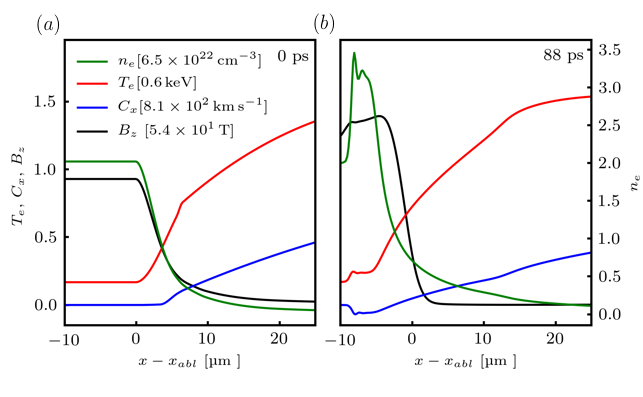
\includegraphics[width=1.0\columnwidth]{pics/one_dim_2col15.png}%
\caption{\label{fig:1Dprof} Lineouts of electron number density, $n_e$, electron temperature, $T_e$, ion flow velocity, $C_x$, and the perpendicular ($z$ direction) magnetic field, $B_z$, for a $\SI{50}{T}$ applied field IMPACT simulation. Initial profiles are presented on the left while right hand side shows lineouts after $\SI{88}{ps}$. }%
\end{figure}

\begin{figure}
	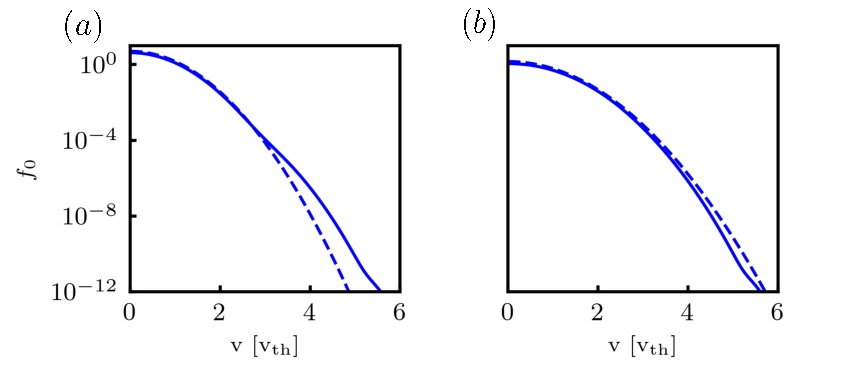
\includegraphics[width=1.0\columnwidth]{pics/f0_50T_LT1_noTe.pdf}%
	\caption{\label{fig:f0prof} Isotropic component of the electron distribution function, $f_0(v)$, sampled from \SI{50}{T} applied field, IMPACT simulation after $\SI{130}{ps}$ of evolution. $f_0$ is displayed at two example points in the conduction zone  (a) at the base of the temperature gradient and (b) at the top of the temperature gradient. Dashed blue line is the equivalent equilibrium form for an electron distribution with the same temperature given for reference. (a) The electron high velocity tail is enhanced relative to equilibrium (b) the high velocity tail is suppressed relative to equilibrium (a dearth of high velocity electrons at the top of the temperature gradient).   Velocity is normalised in terms of the reference thermal velocity, $v_{th}= \sqrt{(2 T_{e,0}/m_e)}$ where $T_{e,0}= \SI{740}{eV}$.} %
\end{figure}


\section{Results}
\subsection{One-dimensional evolution}
\label{sec:1D}
\begin{figure*}
	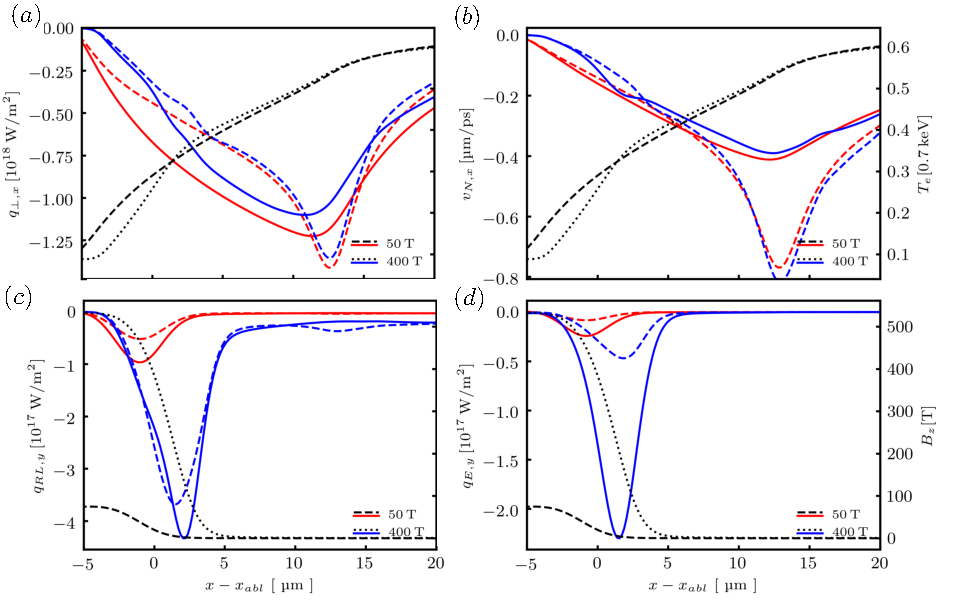
\includegraphics[width=0.8\textwidth]{pics/qlineouts_4plots.pdf}%
	\caption{\label{fig:qlineouts} \label{fig:qperp_1d} Terms driven by $\partial_x T_e$ and $\partial_x B_{z}$. Lineouts of kinetic (solid lines) and classical/local (dashed lines) heat flow  and Nernst components for two different applied field strengths after $\SI{35}{ps}$ of simulation time. Left to right, top to bottom, top, display longitudinal diffusive heat flow, $q_{\perp,x}$ and the longitudinal Nernst velocity, $v_{N,x}$, bottom displays transverse Righi-Leduc heat flow and the transverse thermo-electric heat flow, $q_{E,y}$. Black lines denote lineouts of the temperature and magnetic field for reference. }%
\end{figure*}


In this section, the effect of the applied magnetic field on non-locality and transport is explored in one dimension. The initial profiles and those after \SI{88}{ps} are displayed in Fig. \ref{fig:1Dprof}.  The magnetic field is advected out of the conduction zone and compressed into the ablation surface by the Nernst effect. Figure \ref{fig:f0prof} displays the IMPACT electron distribution function  for a  \SI{50}{T}  simulation.  Fig. \ref{fig:f0prof}(a) displays $f_0(v)$ sampled from a point at the base of the conduction zone temperature gradient while Fig. \ref{fig:f0prof}(b) $f_0(v)$ is taken from the top of the temperature gradient. The relatively collisionless electrons (those with velocities in the range $v=2\,\si{v_{th}}-4\,\si{v_{th}}$), diffuse down the temperature gradient at a much faster rate than their colder, $v \sim \si{v_{th}}$, counterparts.   The high velocity $f_0$ tail becomes depleted at the top of the temperature gradient (b), close to the critical surface and enhanced at the base (a), in the cold dense plasma around the ablation surface, $x\sim \SI{0}{\micro\meter}$. It is well documented that this can cause suppression of transport at the top of the temperature gradient `flux-suppression' and enhancement at the base, for the Nernst term \cite{Brodrick2018,Joglekar2016}, Righi-Leduc heat flow \cite{Kho1985} and diffusive heat flow \cite{Bell1981} (although maybe less of an effect for resistivity \cite{Williams2013}) .

 Figure \ref{fig:qperp_1d} displays lineouts  of the local (assuming thermodynamic equilibrium, dashed lines) and kinetic (solid lines) predictions for transport terms driven by the bulk temperature, $\partial_x T_{e}$, and magnetic field, $\partial_x B_{z}$, gradients in the conduction zone; the diffusive heat flow, $q_{\perp,x}$, Nernst velocity, $v_{N,x}$, transverse Righi-Leduc heat flow, $q_{RL,y}$,  and transverse thermo-electric heat flow, $q_{E,y}$, terms. The solid black line denotes the zeroth order temperature (top) and magnetic field (bottom) profiles for reference. The Nernst and diffusive heat flow deviations from local predictions are qualitatively similar. Non-locality results in a greater than two-fold enhancement of the Righi-Leduc (Fig. \ref{fig:qperp_1d}(c)) and thermo-electric ($\mathbf{q}_{E} = -\dbul{\beta} \cdot \mathbf{j} \frac{T_e}{e}$, Fig. \ref{fig:qperp_1d}(d)) heat flows. This is because these heat flow terms are largest in regions of high magnetic field strength, close to the ablation surface. The regions of high field strength coincide with an enhanced high velocity $f_0$ electron tail, resulting in a corresponding $q_{RL}$ and $q_{E}$ augmentation. 
%  --- transport suppression

Magnetic field restricts the diffusion of electrons perpendicular to its field lines.   Higher velocity electrons, in the distribution function tail, are relatively more magnetised than their thermal counterparts, $\chi = \omega \tau_{ei} \propto v^3$. For the 400 T applied field simulation, the field has been compressed to $\SI{500}{T}$ at the ablation surface by the Nernst effect. This field strength is sufficiently large to `localise' the hot electron preheat at the base of the temperature gradient, $q_{\perp,k}/q_{\perp,c}\rightarrow 1$, close to the ablation surface, $x \sim \SI{0}{\micro\meter}$.  Interestingly, while the Nernst, diffusive heat flow and Righi-Leduc heat flow are effectively localised by this high field strength at $x-x_{abl} \rightarrow 0$, the thermo-electric heat flow, $q_{E,y}$,  blue line in (d) exhibits a 4 fold enhancement relative to its classical counterpart. 


\subsection{Two dimensional Evolution}
\label{sec:2D}
\begin{figure}
	%\includegraphics[width=1.0\columnwidth]{/Users/dominichill/Dropbox/York/UPDATE/PICS_POP/dT_LT1_amp.png}%
		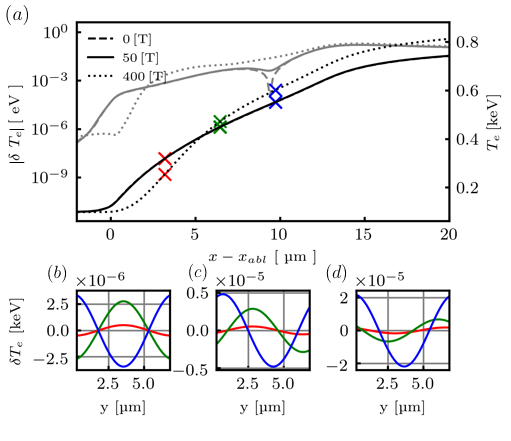
\includegraphics[width=1.0\columnwidth]{pics/plot_dT_4plots_2.png}
	%/Users/dominichill/Dropbox/York/UPDATE/PICS_POP/plot_dT_4plot_LT1_LT1_LT1_06_4plotdT.png
	\caption{\label{fig:dT} (a) $\delta T_e$ (grey lines) and zeroth order $T_e$ (black lines) as a function of distance away from the ablation surface for different applied field strengths (the different line styles). (b), (c) and (d) display lineouts of $\delta T_e$ in the transverse direction, sampled at the corresponding coloured crosses in (a), for a \SI{0}{T} simulation  (b), a \SI{50}{T} applied field simulation (c) and a \SI{400}{T} simulation (d). }%
\end{figure}

%-- Nernst
The Nernst effect efficiently advects magnetic field out of the conduction zone into the cold collisional region around the ablation surface.  As a result, Hall parameters in the conduction zone remain consistently below the $ \chi \sim 0.1$  threshold required to initialise the field-generating thermal or magneto-thermal instabilities. Nevertheless, self-generated fields still play a dominant role in determining the $\delta T_e$ evolution.  Figure \ref{fig:dT}(a) displays the evolution of $\delta T_e$ as a function of distance away from the ablation surface. Lineouts of $\delta T_e(y)$ at various $x-x_{abl}$ positions are presented for the \SI{0}{T}, \SI{50}{T} and \SI{400}{T}  applied field simulations in Fig.s \ref{fig:dT}(b)-(d). Self-generated fields drive a Righi-Leduc heat flow, $\delta q_{y,RL} \propto - \frac{\partial \kappa_{\wedge,0}}{\partial \chi} \partial_x T_{e,0} \delta \chi$, which deflects heat from $\delta \chi$ peaks to troughs. In the \SI{0}{T} and \SI{50}{T} simulations this heat flux inverts the $\delta T_e$ (and thereby the $\delta P_e$) amplitude \cite{Hill2018}. The point at which this phase inversion occurs is indicated by the $|\delta T_e|$ cusp at $x-x_{abl} \approx \SI{10}{\micro\meter}$ in Fig. \ref{fig:dT}(a). The \SI{400}{T} simulation does not exhibit phase inversion. For sufficiently high magnetisation  the direction of  $\delta q_{y,RL}$ reverses ($\frac{\partial \kappa_{\wedge,0}}{\partial \chi} <0$), redirecting heat from $\delta \chi$ troughs to peaks, enhancing the incumbent $\delta T_e$. A linear model for the phase inversion is presented in Section \ref{sec:eigenmodes} and Appendix \ref{app:eigenmodes}.   

In \SI{50}{T} and \SI{400}{T} simulations, the phase of $\delta T_e$ shifts with distance into the conduction zone. This phase shift is predominantly caused by the zeroth order $q_{RL} \propto i k \frac{\partial \kappa_{\wedge,0}}{\partial \chi} \tau_{ei,0} n_0 B_{z,0}\left(l_B - l_n \right)$ (where $l_{\alpha} = \partial_x \alpha_0/ \alpha_0$ and  $\alpha = n_{e}, B_z$), which is driven by the bulk magnetic field and density gradients, redirecting heat in the $y$ direction. 

  % Remark on Cross-gradient Nernst
At the same time, the deflected electrons  responsible for the Righi-Leduc heat flow drag magnetic field lines along with them. This magnetic field advection is the cross-gradient Nernst effect, $\mathbf{v}_{N} = - \beta_{\perp} (\mathbf{b}\times \nabla T_e )$, and is predicted to result in significant magnetic field line twisting in pre-magnetised ICF experiments. %Need citation Walsh2019?  
% put in notes about \partial_t B_z

\subsection{A heuristic model for $\delta T_e$ conduction zone evolution}
\label{sec:eigenmodes}
The  conduction zone evolution of $\delta T_e$ may be explained through linear perturbation theory. The induction equation for the magnetic field and the steady-state temperature equation subject to sinusoidally perturbed heating, $\nabla \cdot \mathbf{q} = (I + \delta Ie^{iky})\delta (x-x_c)$, are used to describe the system. Perturbations in magnetic field and temperature are assumed to take the form, $T_{e} = T_{e,0}(x) + \delta T(x)e^{iky}$, $B_{z} = B_{z,0}(x) + \delta B_z(x)e^{iky}$. Upon linearisng, the following equations  are arrived at, to first order,

\begin{eqnarray}
(\delta_1 + \delta_2 \partial_x^2 )(T_0^{5/2}\delta T) + \epsilon_1 \delta B_{z} &=& 0\label{eq:linear-analysis-Te}\\
(\eta_1 + \eta_2 \partial_x + \eta_3 \partial^2_x)(T_0^{5/2}\delta T) \qquad&& \nonumber\\
+(\gamma_1 +\gamma_2 \partial_x   + \gamma_3 \partial^2_x)\delta B_z&=& 0.\label{eq:linear-analysis-Bz}
\label{eq:linear-analysis}
\end{eqnarray}
where the coefficients are given by,
\begin{eqnarray}
\delta_1 &=& -\kappa_{\perp,0}k^2 + i k \frac{\partial \kappa_{\wedge,0}}{\partial \chi} \tau_{ei,0} n_0 B_{z,0}\left(l_B - l_n \right) \\
\delta_2 &=& \kappa_{\perp,0} \nonumber\\
\epsilon_1 &=& -i k \frac{\partial \kappa_{\wedge,0}}{\partial \chi} \theta_0 T_0^{5/2} \nonumber\\
\eta_1 &=& \frac{i k }{T_0^{5/2}} l_n +\alpha_0
\frac{ B_{z,0}}{T_0^{7/2}}\left(\frac{15}{2} l_T l_B - \frac{3}{2} l_{2,B}\right) + \nonumber\\
&&\frac{\partial \beta_{\wedge,0}}{\partial \chi}\frac{\tau_B B_{z,0}}{n_0 T_0}\left(k^2 + l_B l_T - l_n l_T - 2l_T^2 + l_{2,T} \right) \nonumber\\
\eta_2 &=& - \frac{3}{2}\alpha_0\frac{B_{z,0}}{T_0^{7/2}}l_B + \frac{\partial \beta_{\wedge,0}}{\partial \chi}\frac{\tau_B B_{z,0}}{n_0 T_0} (2l_T + l_n - l_B) \nonumber\\
\eta_3 &=& - \frac{\partial \beta_{\wedge,0}}{\partial \chi} \frac{\tau_B B_{z,0}}{n_0 T_0} \nonumber\\
\epsilon_1 &=& -i k \frac{\partial \kappa_{\wedge,0}}{\partial \chi} \theta_0 T_0^{5/2} 
\end{eqnarray}


\begin{eqnarray}
\gamma_1 &=&\left[ \partial_x C_{x,0} + \alpha_0 k^2 - \frac{\partial \beta_{\wedge,0}}{\partial \chi}\partial_x \theta_0 \right],\nonumber\\
\gamma_2 &=&\left[ C_{x,0} -  \frac{\partial \beta_{\wedge,0}}{\partial \chi}  \theta_0 +\frac{3}{2}\alpha_0 \frac{\partial_x T_0}{T_0} \right ],\nonumber\\
\gamma_3 &=& -\alpha_0, \nonumber \\
\mbox{and } && \nonumber\\
\alpha_0 &=& \frac{\alpha_{\perp,0} \delta_c^2}{T_0^{3/2}}, \quad \theta_0 = \tau_{ei,0}\partial_x T_{0} , \nonumber\\
l_{\zeta} &=& \frac{\partial_x \zeta_0}{\zeta_0} \mbox{ and }\quad  l_{2,\zeta} = \frac{\partial_x^2 \zeta_0}{\zeta_0} \quad(\mbox{where } \zeta = T, B, n). \nonumber
\end{eqnarray}

$n_{0}$, $\kappa_{\perp,0}$, and $\kappa_{\wedge,0}$ represent the zeroth order electron number density, diffusive heat flow coefficient and Righi-Leduc heat flow transport coefficient. The perturbed thermo-electric, $\delta q_{TE}$, heat flow has been neglected here. $\delta q_{TE}$ is significant in regions of both large magnetic field magnitude and gradient which occur close to the ablation surface in the \SI{400}{T} simulation (green line in Fig. \ref{fig:heatflow_phase_shift}), but is negligible in all other conditions simulated here.  The convective transport of heat, $v_{x,0}\partial_x\delta T$ and terms of order $\mathcal{O}(\partial \kappa_{\perp,0}/\partial \chi)$ and above have also been neglected, which are also found to be small.

 The change of variables $\delta u= T_0^{5/2}\delta T$ is made, and the perturbation $x$ dependence is assumed to take the form, $\delta u = \delta u_0 \exp(k_x x)$ and $\delta B_z(x) = \delta B_z \exp(k_x x)$.  It is then possible to find the spatial eigenmodes, $k_x$, of this system, which are well approximated by,
\begin{eqnarray}
k_x &\approx& \left(\frac{(\delta_1 \gamma_1 - \epsilon_1 \eta_1)}{\delta_2 \gamma_3}\right)^{1/4} \nonumber\\
&\approx& \xi k \left[ 1 + \frac{1}{\alpha_0 k^2}\left(\partial_x C_{x,0} - \frac{\partial \beta_{\wedge,0}}{\partial \chi} \theta_0  -\frac{\partial \kappa_{\wedge,0}}{\partial \chi}  \frac{\theta_0 l_n}{ \kappa_{\perp,0}} \right)\right.  \nonumber\\
&  & \left. +\frac{i}{\kappa_{\perp,0}\alpha_{0} k}  \frac{\partial \kappa_{\wedge,0}}{\partial \chi} \tau_{ei,0} n_0 B_{z,0}\left( l_B - l_n \right) \right]^{1/4},
\label{eq:eigenvalues}
\end{eqnarray}
where $\xi = +1, -1, +i, -i$. A full derivation of Eq. \ref{eq:eigenvalues} and the related $\delta u$ and $\delta B_z$ eigenfunctions is given in Appendix \ref{app:eigenmodes}. The first term in the numerator represents the coupling between magnetic field amplification and damping (caused by the  Nernst effect, frozen in flow and resistivity) and the diffusive damping of the temperature perturbation. The second term in the numerator, $\epsilon_1 \eta_1$,  is the instability or mode inversion source term, the coupling between spontaneous generation of magnetic field by the Biermann-battery effect, $\eta_1$, and the Righi-Leduc heat flow, $\epsilon_1$. 


The magnitude and phase of $k_x$ vary depending on the degree of magnetisation. 
If all magnetic field effects are neglected, Eq. \ref{eq:linear-analysis} reduces to a diffusion equation describing thermal smoothing of $\delta T$ via diffusive thermal conduction, $k_x \rightarrow k$. This limit describes the exponential attenuation of $\delta T_e$ with distance into the conduction zone, sometimes referred to as the `cloudy day' thermal smoothing model  \cite{Nuckolls1972,Goncharov2006}. 

The coupling between Righi-Leduc and self-generated fields, $\epsilon_1 \eta_1 $, is pivotal in the perturbation evolution. $\epsilon_1 \eta_1$, changes sign depending on whether $\chi$ is less than or greater than $\sim 0.1$ (this threshold depends on $Z$ through its dependence  on $\frac{\partial \kappa_{\wedge,0}}{\partial \chi}$). 

 For  $\chi \gtrsim 0.1$, as is the case in the \SI{400}{T} simulation,  $\frac{\partial \kappa_{\wedge,0}}{\partial \chi}<0$ and $\epsilon_1 \eta_1>0$, (according to local predictions) \cite{Epperlein1986}, and this term results in a smaller $k_x$ and thus either slower $\delta T_e$ or $\delta B_z$ damping or growth due to field-generating thermal or magneto-thermal instabilities.

In the opposing limit (relevant for \SI{0}{T} and \SI{50}{T}), $\epsilon_1 \eta_1 < 0$. In this case the $\epsilon_1 \eta_1$ term acts to damp the incumbent $\delta T$. Unlike conventional damping, the damping term is driven by the 10-100 fold $\delta B$ amplification by the Nernst effect within the conduction zone. Instead of returning to zero, the $\delta T_e$  overshoots and inverts \cite{Hill2018}, seen in the green and red curves of Fig. \ref{fig:dT}(b).  In Appendix \ref{app:eigenmodes} analysis of the system Eigenmodes is used to show that $\delta T_e$ perturbation is composed of both a decaying and an oscillatory component, the latter of which is responsible for this phase inversion.
%-------------------------------------------

\subsection{Non-locality and magnetic field self-generation and Righi-Leduc heating }
\label{sec:biermann_and_qrl}
In the previous section we explored how the limits of $\delta T_e$ (and therefore $\delta P$) evolution, instability and `overdamping', are governed by the interplay between  $\delta q_{RL,y}$, $\partial_t B$ generation and the Nernst advection of the B-field. 

In this section we investigate the manner in which non-locality may affect these two sides of the magneto-thermal and field-generating thermal instability feedback loops.  Fig.  \ref{fig:qrl_contour} and Fig. \ref{fig:bier_contour} display colour maps of the perturbed Hall parameter $\delta \chi = \chi - \langle \chi \rangle$ overlayed with contours of Righi-Leduc heating, $\partial_y q_{y,RL}$ and magnetic field amplification and advection, due to the Biermann and cross-gradient Nernst term, $\partial_t B_{z,1}$,  given by the expression,
\begin{eqnarray}
\partial_t \mathbf{B} &= \nabla \times\left( \frac{\nabla P_e}{e n_e} + \frac{1}{e} \dbul{\beta}^c \cdot \nabla T_e  \right)\nonumber\\
&= - \frac{\nabla n_e \times \nabla T_e}{e n_e} + \nabla \times (\mathbf{v_{\wedge} } \times \mathbf{B})
\end{eqnarray}
where $\mathbf{v}_{\wedge} = \frac{\beta^c_{\perp}}{e |\mathbf{B}|}\nabla T_e$.  Figures \ref{fig:qrl_contour}(a) and \ref{fig:bier_contour} (a) correspond to a $\SI{50}{T}$ applied field simulation while Fig.s \ref{fig:qrl_contour}(b) and \ref{fig:bier_contour}(b) are a $\SI{400}{T}$ simulation. Green contours are the predicted values for $\partial_y q_{RL,y}$ and $\partial_t B_{z}$ given by a local model, while red contours are those of the true non-local values, reconstructed from the IMPACT simulations.

 $\SI{50}{T}$ and $\SI{400}{T}$ simulations show several key differences.  In the  $\SI{50}{T}$  case, at the peak of the temperature gradient  $\partial_y q_{RL,y}$ heats $\delta \chi $ troughs ($\pi$ out of phase) in Fig. \ref{fig:qrl_contour}, causing the $\delta T$ amplitude to invert, but is in phase with $\delta \chi$ in the $\SI{400}{T}$ case, instead growing the incumbent $\delta T$. Further into the conduction zone contours of $\partial_t B_{z}$ and $\partial_y q_{y,RL}$ twist, shifting in the y direction, due to a combination of $v_{N,\wedge}$ magnetic field advection and the $\partial_x B_{z}$ and $\partial_x n_0$ driven Righi-Leduc heat flow $q_{RL} \propto i k \frac{\partial \kappa_{\wedge,0}}{\partial \chi} \tau_{ei,0} n_0 B_{z,0}\left(l_B - l_n \right)$ .

Comparison of green (local) and red (non-local) contours  demonstrates that Righi-Leduc heating is larger in a non-local model for both applied field strengths (the $+\sigma$ and $-\sigma$ contours extend over a much wider area). A possible explanation for this is that the Righi-Leduc heat flow is mediated by a more magnetised hot electron population ($\chi = \omega \tau_{ei}(v) \propto v^3$). Therefore, the electron deficit in the $f_0$ tail is compensated for by an increase in effective magnetisation, resulting in a net $q_{y,RL}$ enhancement even at the top of the temperature gradient.   Biermann field generation and cross-gradient Nernst advection, on the other hand, are reduced by non-locality in regions of flux-suppression. 

Close to the ablation surface, non-local and local contours of $\partial_y q_{RL,y}$ are offset in the $\SI{50}{T}$ simulation (Fig. \ref{fig:qrl_contour}(a)), but nearly exactly overlap in the $\SI{400}{T}$ simulation (Fig. \ref{fig:qrl_contour}(b)). This is likely due to the $x\sim x_{abl}$ magnetic field creating a transport barrier which localises $q_{RL,y}$, consistent with results seen in Fig. \ref{fig:qlineouts}.
% Final point

%dyqyRL_contour_wt_im_lt1_11.png
\begin{figure}
	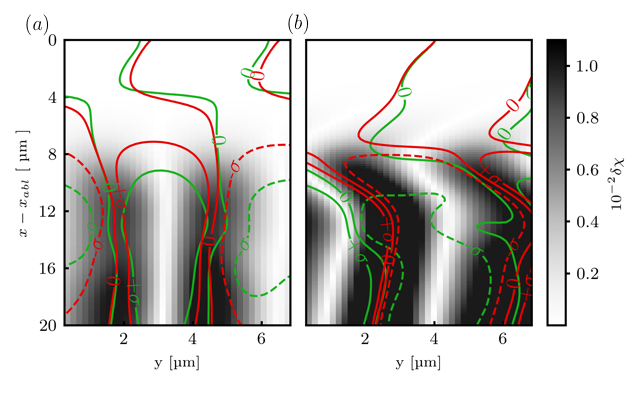
\includegraphics[width=1.0\columnwidth]{pics/plot_dqy_qRL_contour_11_LT1_100p_green.png}
	\caption{\label{fig:qrl_contour} Image plots of $\delta \chi$ within the conduction zone with $\partial_y q_{y,RL}$ contours overlayed for simulations with $\si{50}{T}$ (left) and a $\si{400}{T}$ (right) applied magnetic fields. Three contours are plotted, $-\sigma$, $0$, and $+\sigma$. Red and green contours are values for $\partial_y q_{y,RL}$ reconstructed from IMPACT simulations and as predicted by a local model respectively. }
\end{figure}

\begin{figure}
	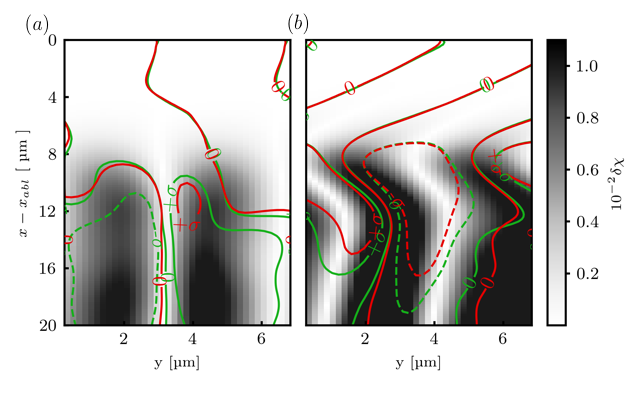
\includegraphics[width=1.0\columnwidth]{pics/plot_dqy_bier_contour_11_LT1_100p_green.png}
	\caption{\label{fig:bier_contour} Image plots of $\delta \chi$ within the conduction zone with $\partial_t \mathbf{B}$ contours overlayed for simulations with $\si{50}{T}$ (left) and a $\si{400}{T}$ (right) applied magnetic fields.   Three contours are plotted, $-\sigma$, $0$, and $+\sigma$, red is kinetic (reconstructed from IMPACT simulations) while green is the local predictions for $\partial_y q_{y,RL}$. }
\end{figure}


\begin{figure*}
		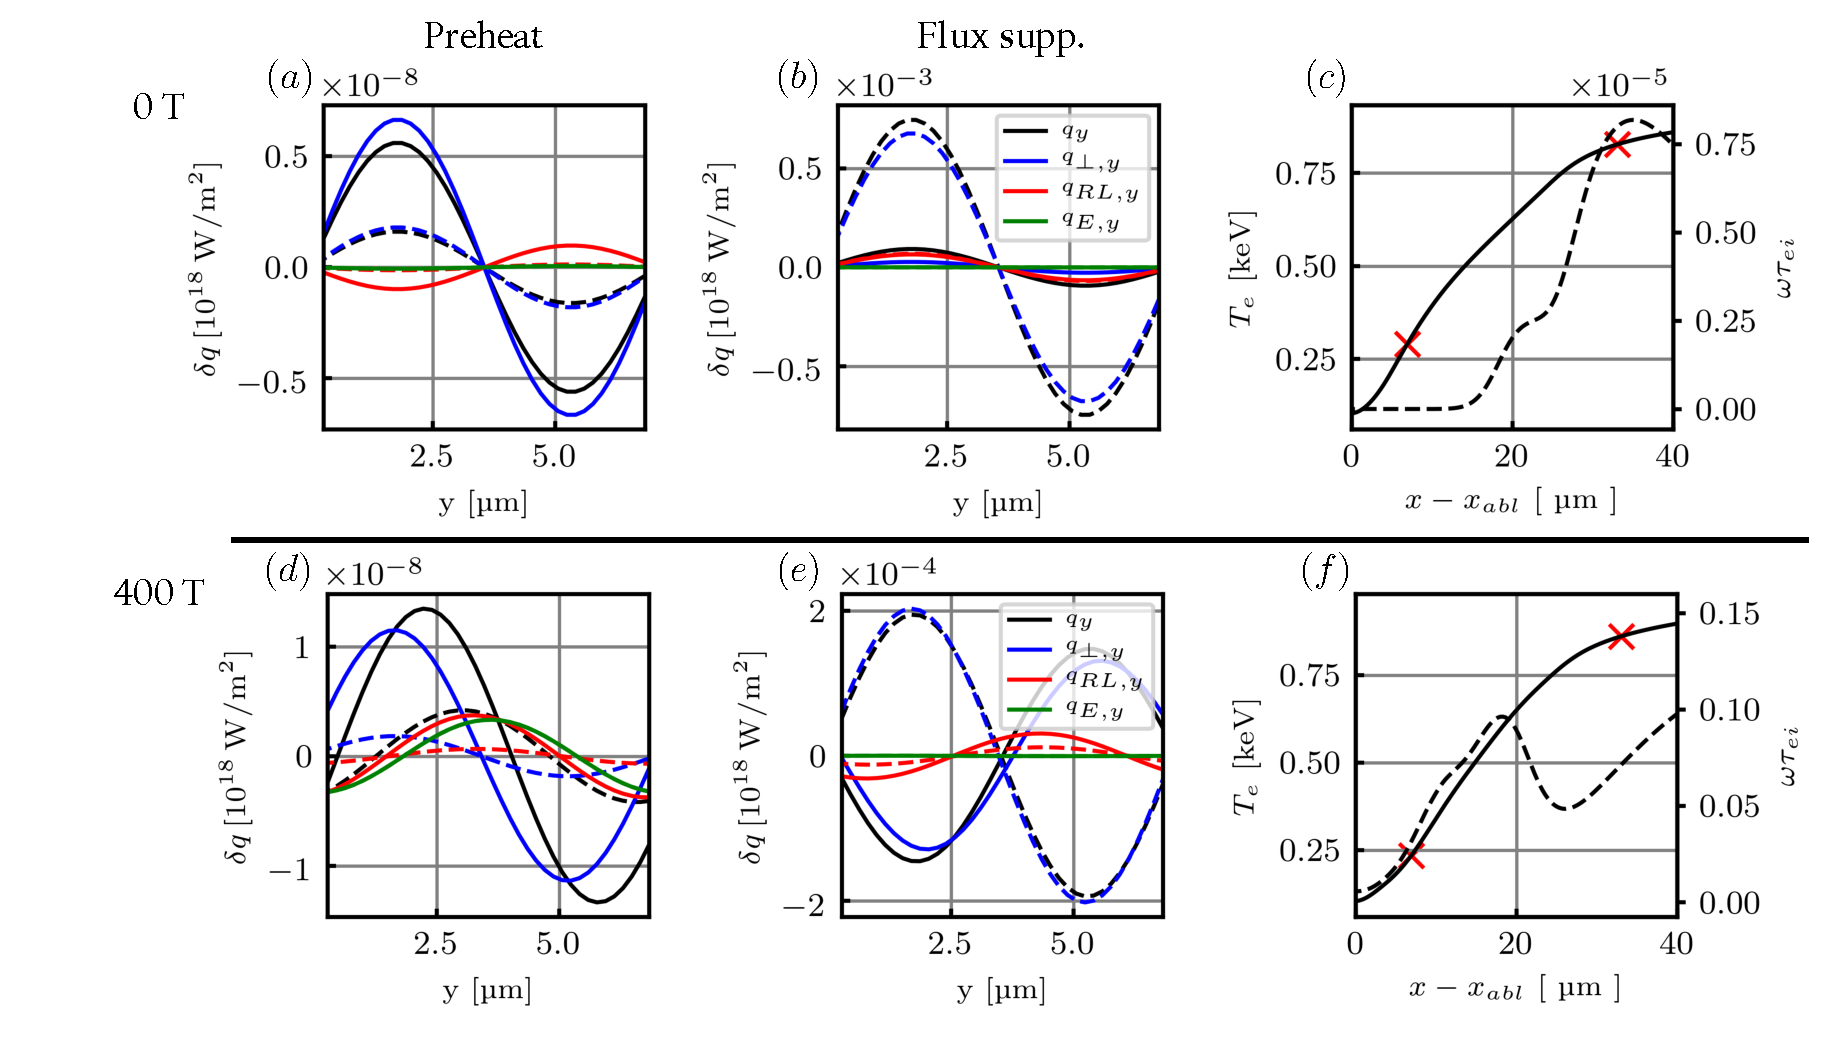
\includegraphics[width=1.0\textwidth]{pics/dqy_LT2_0T_400T_2.pdf}
	\caption{\label{fig:heatflow_phase_shift} Lineouts of $\delta q_{y}$ at different positions in the conduction zone. Left, a region of preheat, right a region of flux-suppression, sampled at positions marked by the left and right crosses on the temperature gradient on the right hand side respectively. Solid lines represent kinetic predictions for each heat flow component while dashed lines represent local thermodynamic equilibrium components. In (a) $\delta q_{y}$ (solid blue line) is both enhanced and shifted out of phase by $-\pi/2$ relative to the local prediction, dashed blue line. While in (b) heat flow is suppressed }
\end{figure*}

\subsection{The effect of non-locality on the transverse heat flow}
\label{sec:non-locality-2D}
%--- 

Non-locality changes both the magnitude and direction of the heat flux. The latter is investigated in this section. Correct determination of heat flux direction is important as the relative degree of transverse heat flow governs both the thresholds for instability and thermal smoothing magnitudes. 

Non-local modification of the heat flow and Nernst-effect  directions is primarily due to two mechanisms here. The first is that was originally studied by Epperlein et al. in VFP simulations without B-field \cite{Epperlein1988}. Hot, long $\lambda_{mfp}$ electrons are only sensitive to relatively long scale length changes in plasma temperature and collisionality. These long $\lambda_{mfp}$ electrons are relatively, unperturted by the local, short scale length, modulations in the transverse direction compared to bulk gradients. The resultant heat flow and Nernst effects are directed much further down the bulk temperature gradient,  shown schematically in Fig. \ref{fig:heat_flow_rotation}. The Righi-Leduc heat flow, which is $q_{RL} \propto -(\mathbf{b} \times \nabla T_e)$,   rotates in the opposite direction (further towards the transverse direction). Furthermore, in regions of preheat, effects of non-locality reverses the roles of the arrows: $q_{\perp}$ and $v_N$ are enhanced and rotated further in the transverse direction while $q_{RL}$ is enhanced and rotated further down the temperature gradient. The rotation displayed in Fig. \ref{fig:heat_flow_rotation} applies for cases of low magnetisation ($\SI{0}{T}$ and $\SI{50}{T}$). For larger applied field strengths non-local direction changes are controlled by the second mechanism.

The second mechanism is caused by the differing magnetisation of hot electron populations (relative to the thermal Hall parameter). Magnetic field, changes the magnitude of coefficients within, the transport tensors of Eq. \ref{eq:transport}, hence a changing effective magnetisation will also alter the prevailing direction of heat flux and Nernst advection.

\begin{figure}
	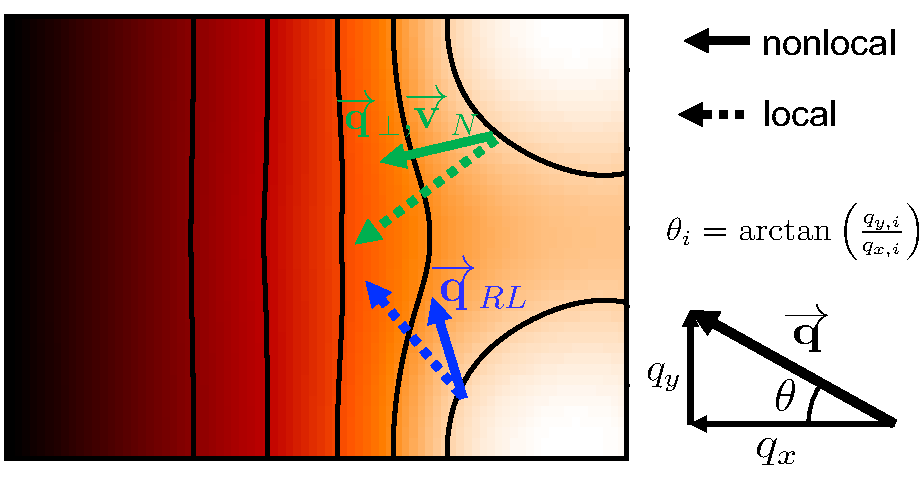
\includegraphics[width=1.0\columnwidth]{pics/heatflow_angle_schematic.pdf}
	\caption{\label{fig:heat_flow_rotation} Schematic showing the manner in which non-locality rotates and changes the magnitudes of different transport terms $q_{\perp}$, $v_N$ and $q_{RL}$. In regions of preheat, the dashed and solid arrows reverse in characteristic - the Nernst and diffusive heat flow become larger and further towards the transverse direction than their equilibrium counterparts. While the Righi-Leduc heat flow becomes larger and rotates further down the temperature gradient. }
\end{figure}

The change of direction in turn, acts to alter the phase of $\delta q$. Figure \ref{fig:heatflow_phase_shift} displays lineouts of $\delta q$ for the different heat flow components. The degree to which non-locality shifts the phase of different $\delta q_y$ components is a function of the distribution function shape and their relative sensitivity to magnetisation effects.  Two characteristic points in the conduction zone are selected, for two different strengths of externally applied magnetic field, $\SI{0}{T}$ and $\SI{400}{T}$. Figures \ref{fig:heatflow_phase_shift}(a) and \ref{fig:heatflow_phase_shift}(d), the region of preheat, Fig.s \ref{fig:heatflow_phase_shift}(b) and \ref{fig:heatflow_phase_shift}(e), a point of `heat flux-suppression' at the top of the temperature gradient. 

As expected $\delta q$ exhibits non-local suppression and enhancement in all heat flow components in regions of flux-suppression and preheat respectively for $\SI{0}{T}$ simulations. The same is not true in $\SI{400}{T}$ simulation.  
The perturbed Righi-Leduc heat flow shows non-local enhancement of its amplitude even in regions of flux-suppression.  Meanwhile, nonlocality has shifted the relative phase of $\delta q$ for various heat flow components. In the most extreme example, the non-local $\delta q_y$ (solid black line) is directed in the opposite direction to local predictions (dashed black line) for the $\SI{400}{T}$ simulation at the top of the temperature gradient, Fig. \ref{fig:heatflow_phase_shift}(e).







\section{Summary and Conclusions}
There has been growing interest in performing laser-ablation experiments that involve a pre-applied magnetic field. Conditions within the conduction zone of ablating laser-plasmas are fundamentally non-local. Full integrated kinetic modelling of semi-collisional plasmas is outside the scope of current computational resources, as a result it is standard to include a reduced model of non-local effects into integrated hydrodynamics modelling of laser plasmas. Reduced non-local models currently lack benchmarking in more than one spatial dimension and within magnetised environments. It therefore remains important to understand the variety of ways in which non-locality may modify transport from predictions made using conventional hydrodynamics modelling.

Two dimensional Vlasov-Fokker-Planck simulations of the conduction zone of pre-magnetised ICF targets have been performed. The Nernst effect rapidly cavitates the conduction zone magnetic field, as a consequence only relatively modest $\omega \tau_{ei} \lesssim 0.2$ Hall parameters are achieved in these simulations.  As a consequence the onset of magneto-thermal and Tidman Shanny instabilities is inhibited in simulations presented here, even for large applied magnetic field strengths (up to $\SI{400}{T}$). Two limits of temperature perturbation evolution are explored. 

In the low magnetisation limit, $L_n \frac{\partial \kappa_{\wedge,0}}{\partial \chi} \partial_x T_0 < 0$, the Righi-Leduc heat flows down gradients of Hall parameter, inverting the perturbation and causing its amplitude to oscillate with distance into the conduction zone. In the high magnetisation limit, $L_n \frac{\partial \kappa_{\wedge,0}}{\partial \chi} \partial_x T_0 < 0$, the Righi-Leduc heat flow behaves as a source term for the MTI and TSI. $\delta q_{RL,y}$ instead directs heat towards $\delta \chi$ peaks, competing with the damping effects of diffusive thermal conduction to increase the $\delta T$ amplitude. For the $\SI{400}{T}$ simulation this results in both suppression of phase inversion and a larger ablation surface $\delta T_e$ relative to $\SI{0}{T}$ and $\SI{50}{T}$. However,  a net growth in $\delta T$,  caused by instability, does not occur.


Non-local effects alter these processes. The hot, relatively collisionless electrons ($\lambda_{mfp} \propto v^4$, where $v$ is the electron velocity) stream down the temperature gradient resulting in a hot electron population deficit close to the critical surface and an enhanced population at the ablation surface.  As a rule of thumb, this fast-electron population surplus and deficit causes a corresponding increase and reduction in the extended-magnetised transport terms, including Nernst, diffusive heat flow and Biermann battery magnetic field spontaneous generation/ cross-gradient Nernst advection. However, this general rule is not always true when an applied magnetic field is present. For large applied magnetic fields, the magnetic field which is advected towards the ablation surface and compressively amplified, forms a transport barrier acting to `localise’ transport in this region. Meanwhile, the Hall parameter scales with the electron velocity, $\omega \tau_{ei} \propto v^{3}$. For magnetised transport terms (eg. $q_{y,RL}$ \cite{Kho1985}) mediated by high velocity, more magnetised electrons the \emph{effective magnetisation} of the plasma transport may be much higher than the thermal electrons' Hall parameter. In the $\SI{50}{T}$ simulation, this effect results in an enhanced $q_{RL,y}$ relative to local models, even at the top of the temperature gradient, in the region typically assigned for flux-suppression. 


\section{Appendix}

\label{app:eigenmodes}
Linear perturbation theory may be used to describe the conduction zone spatial evolution of $\delta T_e$. Starting with the steady-state temperature equation, subject to sinusoidally perturbed heating, $\nabla \cdot \mathbf{q} = I\delta (x-x_c)$, assuming harmonic perturbations in magnetic field and temperature of the form,
\begin{eqnarray}
\delta T &\propto \delta T e^{iky + i \omega t + k_x x}\\
\delta B_z &\propto \delta B_z e^{iky + i \omega t + k_x x},
\end{eqnarray}
the following linearised temperature and magnetic field equations are arrived at,
\begin{eqnarray}
&(\delta_1 + \delta_2 \partial_x^2 )\delta u &+ \epsilon_1 \delta B_{z} = 0\\
&(\eta_1 + \eta_2 \partial_x + \eta_3 \partial^2_x)\delta u &+(\gamma_1 + \gamma_2 \partial_x + \gamma_3 \partial^2_x)\delta B_z= 0,
\end{eqnarray}
where the coefficients are defined as follows,

\begin{eqnarray}
\delta_1 &=& -\kappa_{\perp,0}k^2 + i k \frac{\partial \kappa_{\wedge,0}}{\partial \chi} \tau_{ei,0} n_0 B_{z,0}\left(l_B - l_n \right) \\
\delta_2 &=& \kappa_{\perp,0}
\end{eqnarray}

\begin{eqnarray}
\eta_1 &=& \frac{i k }{T_0^{5/2}} l_n +\alpha_0
\frac{ B_{z,0}}{T_0^{7/2}}\left(\frac{15}{2} l_T l_B - \frac{3}{2} l_{2,B}\right) + \nonumber\\
&&\frac{\partial \beta_{\wedge,0}}{\partial \chi}\frac{\tau_B B_{z,0}}{n_0 T_0}\left(k^2 + l_B l_T - l_n l_T - 2l_T^2 + l_{2,T} \right)\\
\eta_2 &=& - \frac{3}{2}\alpha_0\frac{B_{z,0}}{T_0^{7/2}}l_B + \frac{\partial \beta_{\wedge,0}}{\partial \chi}\frac{\tau_B B_{z,0}}{n_0 T_0} (2l_T + l_n - l_B) \\
\eta_3 &=& - \frac{\partial \beta_{\wedge,0}}{\partial \chi} \frac{\tau_B B_{z,0}}{n_0 T_0}
\end{eqnarray}

\begin{equation}
\epsilon_1 = -i k \frac{\partial \kappa_{\wedge,0}}{\partial \chi} \theta_0 T_0^{5/2} 
\end{equation}


\begin{eqnarray}
\gamma_1 &=&\left[ \partial_x C_{x,0} + \alpha_0 k^2 - \frac{\partial \beta_{\wedge,0}}{\partial \chi}\partial_x \theta_0 \right],\nonumber\\
\gamma_2 &=&\left[ C_{x,0} -  \frac{\partial \beta_{\wedge,0}}{\partial \chi}  \theta_0 +\frac{3}{2}\alpha_0 \frac{\partial_x T_0}{T_0} \right ], \nonumber\\
\gamma_3 &=& -\alpha_0, \nonumber\\
\mbox{where} && \nonumber\\
\alpha_0 &=& \frac{\alpha_{\perp,0} \delta_c^2}{T_0^{3/2}}, \quad \theta_0 = \tau_{ei,0}\partial_x T_{0} , \nonumber\\
l_{\zeta} &=& \frac{\partial_x \zeta_0}{\zeta_0} \mbox{ and }\quad  l_{2,\zeta} = \frac{\partial_x^2 \zeta_0}{\zeta_0} \quad(\mbox{where } \zeta = T, B, n). \nonumber
\end{eqnarray}

The eigenmodes of this system are given by the quartic equation,

\begin{eqnarray}
\label{eq:disprel}
\delta_2 \gamma_3 k_x^4 + \delta_2 \gamma_2 k_x^3 + (\delta_1 \gamma_3 + \delta_2 \gamma_1 - \epsilon_1 \eta_3 ) k_x^2  \nonumber\\
 + (\delta_1 \gamma_2 - \epsilon_1 \eta_2) k_x + (\delta_1 \gamma_1 - \epsilon_1 \eta_1) = 0.
\end{eqnarray}
For the case $l_B > l_T$ the $k_x^3$, $k_x^2$ and $k_x$ coefficients are small and Eq. \ref{eq:disprel} has the approximate solutions,

\begin{eqnarray}
k_x &\approx& \left(\frac{(\delta_1 \gamma_1 - \epsilon_1 \eta_1)}{\delta_2 \gamma_3}\right)^{1/4} \nonumber\\
&\approx& \xi k \left[ 1 + \frac{1}{\alpha_0 k^2}\left(\partial_x C_{x,0} - \frac{\partial \beta_{\wedge,0}}{\partial \chi} \theta_0  -\frac{\partial \kappa_{\wedge,0}}{\partial \chi}  \frac{\theta_0 l_n}{ \kappa_{\perp,0}} \right)\right.  \nonumber\\
&  & \left. +\frac{i}{\kappa_{\perp,0}\alpha_{0} k}  \frac{\partial \kappa_{\wedge,0}}{\partial \chi} \tau_{ei,0} n_0 B_{z,0}\left( l_B - l_n \right) \right]^{1/4}
\label{eq:eigenvalues2}
\end{eqnarray}
where $\xi = +1, -1, +i, -i$. The first term in the numerator represents the coupling between magnetic field amplification and damping (caused by the  Nernst effect, frozen in flow and resistivity) and the diffusive damping of the temperature perturbation. The second term  is the instability or mode inversion source term, composed of the coupling between the spontaneous generation of magnetic field by the Biermann-battery effect and the Righi-Leduc heat flow. The final term on the right hand side is responsible for shifting the phase of the $\delta T_e$, and is negligible in $\SI{50}{T}$ simulations except for regions close to the ablation surface. 
\mypara

In the limit that all magnetic field and hydrodynamic effects are neglected the cloudy day model is recovered $k_x \rightarrow k$ \cite{Bodner1974}.

For the case of Dirichlet boundary conditions bounding the conduction zone, $\delta T(x_c) = \delta T_{c}$ and $\delta B_{z}(x_c) \rightarrow \delta B_{z,c}$, and $\delta T(x_c) \rightarrow 0$ $\delta B_z(x_a) \rightarrow 0$  at the ablation surface (suitable for early times) we find that eigenvalues in Eq. \ref{eq:eigenvalues}, yield the solution,

 \begin{equation}
 \delta T_{e} = (c_{1,r} + i c_{1,i}) \sinh(k_x x) + (c_{2,r} + i c_{2,i}) \sin (k_x x)
\end{equation}
where, 
\begin{eqnarray}
c_{1,r} &= \frac{1}{2k_x^2 T_0^{5/2}}(k_x^2 - k^2) u_c \mbox{sech}(k_x x_c) \\
c_{1,i} &= \frac{\delta B_{z,c} \kappa_{\perp,0}}{2k_x ^2 \zeta T_0^{5/2} }(k_x^4 - k^4 ) \mbox{sech}(k_x x_c)\\
c_{2,r} &= \frac{\delta B_{c} \kappa_{\perp,0}}{2k_x^2 \zeta T_0^{5/2}}(k^4 -k_x^4) \mbox{sech}(k_x x_c)\\
c_{2,i} &= \frac{1}{2k_x^2 T_0^{5/2}}(k^2 +k_x^2) u_c \mbox{sech}(k_x x_c)\\
\end{eqnarray}

where $\zeta = -i\epsilon_1$.








% Tables may be be put in the text as floats.
% Here is an example of the general form of a table:
% Fill in the caption in the braces of the \caption{} command. Put the label
% that you will use with \ref{} command in the braces of the \label{} command.
% Insert the column specifiers (l, r, c, d, etc.) in the empty braces of the
% \begin{tabular}{} command.
%
% \begin{table}
% \caption{\label{} }
% \begin{tabular}{}
% \end{tabular}
% \end{table}

% If you have acknowledgments, this puts in the proper section head.
%\begin{acknowledgments}
% Put your acknowledgments here.
%\end{acknowledgments}

% Create the reference section using BibTeX:
%\bibliography{your-bib-file}
\bibliography{bib/library}



\end{document}

%
% ****** End of file aiptemplate.tex ******